\section{Berry phase}
    Berry phase is the simplest demonstration of how geometry and topology can emerge from quantum mechanics and at heart of the quantum Hall effect.\newline
    Let us consider a physical system described by a Hamiltonian that depends on a set of parameters $\boldsymbol \lambda=(\lambda_1,\lambda_2,\dots)$. These parameters do not represent the degrees of freedom of the system like position and momentum, rather they describe things such as the mass of a particle, the strength of a potential and so on.\\ For each $H(\boldsymbol \lambda)$ there exists a set of eigenstates such that 
    \begin{equation}
        H(\boldsymbol \lambda)\ket{n,\boldsymbol \lambda}=E_n(\boldsymbol \lambda)\ket{n,\boldsymbol \lambda}
    \end{equation}
    However the equation above does not completely determine the basis function $\ket{n,\boldsymbol \lambda}$; We can change arbitrarily the phase $\gamma_n(\boldsymbol \lambda)$ of any eigenstate which is called \textit{Berry phase}
    \begin{equation}
        \label{eq:berryphase}
        \ket{n,\boldsymbol \lambda}\to \underbrace{e^{i\gamma_n(\boldsymbol \lambda (t))}}_{\textrm{Berry phase}} \ket{n,\boldsymbol \lambda}  
    \end{equation}
    Suppose we start off with a Hamiltonian and then we slowly change the parameters for a time $T$ until it reaches a different Hamiltonian, this means that $\boldsymbol \lambda=\boldsymbol \lambda(T)$. For the adiabatic theorem we can say that if we start on an energy eigenstate, and the system changes slowly enough,
    \footnote{How slow you have to be in changing the parameters depends on the energy gap from the state you're in to the nearest other state. The smaller the gap, the slower you have to change the parameters. A way of showing this without doing long calculations is the following: \\ We know from the Heisenberg uncertainty principle that $T \Delta E \ge \hbar/2$. We want the uncertainty in the Energy to be way smaller than the energy gap $E_g \gg\Delta E$, so $E_g \gg \frac{\hbar}{2T}$, therefore if we make $T$ big enough it can be achieved}
    and has no degeneracies, then the system will cling on that energy eigenstate.\newline
    This means that the equation of motion of a particle that for time $t=0$ is equal to $\ket{\psi_n(t=0)}=\ket{n,\boldsymbol \lambda(0)}$ is 
    \begin{equation}
        \label{eq:psin}
        |\psi_n(t)\rangle=\underbrace{e^{i\gamma_n(\boldsymbol \lambda (t))}}_{\textrm{Berry phase}}\cdot
        \underbrace{e^{-\frac i\hbar\int_0^t E_n(\boldsymbol \lambda (t')) dt'}}_\textrm{dynamical phase}|n,\boldsymbol \lambda (t)\rangle      
    \end{equation}
    Where the first exponent comes from eq. \ref{eq:berryphase}. We now insert the equation above into the time-dependent Shrodinger equation
    \begin{equation}
        \label{eq:shrodt}
        i\hbar\partial_t|\psi_n(t)\rangle=H(\boldsymbol \lambda(t)) |\psi_n(t)\rangle
    \end{equation}
    By plugging equation \ref{eq:psin} into the \textit{right} term term of equation \ref{eq:shrodt} we get we get that
    \begin{equation}
        \label{eq:H(t)}
        H(\boldsymbol \lambda(t)) |\psi_n(t)\rangle = E_n(t)\ket{\psi_n(t)}
    \end{equation}
    Andy By plugging equation \ref{eq:psin} into the \textit{left} term term of equation \ref{eq:shrodt} we get we get that

    \begin{equation}
        \label{eq:psin-t}
        i\hbar\partial_t|\psi_n(t)\rangle=
        -\hbar \dot \gamma_n(t)|\psi_n(t)\rangle + E_n(t)|\psi_n(t)\rangle + e^{i\phi_n(t)}\partial_t|n,t\rangle
    \end{equation}
    where we have defined $e^{i\phi_n(t)} \equiv e^{i\gamma_n(\boldsymbol \lambda (t))}e^{-\frac i\hbar\int_0^t E_n(\boldsymbol \lambda (t')) dt'}$

    By equating the right terms in equations \ref{eq:H(t)} and \ref{eq:psin-t} we get that 
    \begin{equation}
        \label{eq:psin-t-H}
            i\hbar e^{i\phi_nt(t)}\partial_t|n,t\rangle=\hbar\dot \gamma_n(t)\ket{\psi_n(t)} =\hbar\dot \gamma_n(t)e^{i\phi_n(t)}\ket{n,t}
    \end{equation}    
    now we multiply the term on the left and on the right of equation \ref{eq:psin-t-H} by $\hbar^{-1}e^{-i\phi_n(t)} \bra{n,t}$
    \begin{equation}
        \label{eq:psin-t-H-bra}
            \dot \gamma_n(t)=i\bra{n,t} \partial_t\ket{n,t}
    \end{equation}
    We can re-express it in terms of $\boldsymbol \lambda$
    \begin{equation}
        \label{eq:connection}
            \dot \gamma_n(t)=\dot{\boldsymbol \lambda}\cdot\underbrace{i\bra{n,t} \partial_{\boldsymbol \lambda}\ket{n,t}}_{\equiv \mathbf A_n(\boldsymbol \lambda)}
    \end{equation}
    Where $\mathbf A_n(\boldsymbol \lambda)$ called the \textbf{Berry connection}
    This means that we can calculate the total change in $\gamma_n(t)$ can be obtained by doing a line integral in the space of parameters $\boldsymbol \lambda$ over the path $\mathcal P$ of values that $\boldsymbol \lambda$ assumes during the time evolution

    \begin{equation}
        \label{eq:line_int1}
            \gamma_n=\int_\mathcal{P} \mathbf A_n(\boldsymbol \lambda) \cdot d\boldsymbol \lambda
    \end{equation}


    \begin{equation}
        \label{eq:re-define}
        \ket{n,\boldsymbol \lambda}\to e^{if_n(\boldsymbol \lambda)}\ket{n,\boldsymbol \lambda}
    \end{equation}

    Keep in mind however that the eigenstates are defined up to a phase, meaning that we can re-define the base vectors like so 
    (equation \ref{eq:re-define}). If we apply this substitution into the formula of $\mathbf A_n$ we have that

    \[
    \mathbf A_n(\boldsymbol \lambda) =i\bra{n,t} \partial_{\boldsymbol \lambda}\ket{n,t}\to i\bra{n,t} \partial_{\boldsymbol \lambda}\ket{n,t} - \partial_{\boldsymbol \lambda}f_n(\boldsymbol \lambda)
    \]

    \begin{equation}
        \label{eq:gauge1}
        \mathbf A_n \to \mathbf A_n - \partial_{\boldsymbol \lambda}f_n
    \end{equation}
        So the system is invariant under the gauge transformation in equation \ref{eq:gauge1}. If we do this transformation to equation \ref{eq:line_int1} we have that

    \[
        \gamma_n=\int_\mathcal{P} \mathbf A_n(\boldsymbol \lambda) \cdot d\boldsymbol \lambda - \int_\mathcal{P} \partial_{\boldsymbol \lambda}f_n(\boldsymbol \lambda) \cdot d\boldsymbol \lambda= \int_\mathcal{P} \mathbf A_n(\boldsymbol \lambda) \cdot d\boldsymbol \lambda + f(\boldsymbol \lambda(0))-f(\boldsymbol \lambda (T))
    \]
    This means that if the path $\mathcal{P}$ is open we can always choose a function $f_n$ such that 
    $f(\boldsymbol \lambda(0))-f(\boldsymbol \lambda(T))=\int_\mathcal{P} \mathbf A_n(\boldsymbol \lambda) \cdot d\boldsymbol \lambda$, 
    thus we can conclude that one can always choose a suitable $f(\boldsymbol \lambda)$ such that $\gamma_n$ accumulated along the path $\mathcal P$ is calceled out leaving equation 
    \ref{eq:psin} with only the dynamical phase. 
    However if the path is closed $\boldsymbol \lambda(0)=\boldsymbol \lambda(T)$, in order to make the phase change
    in equation \ref{eq:re-define} single value we must have that
    \[
    e^{f(\boldsymbol \lambda(0))-f(\boldsymbol \lambda(T))}=1
    \]
    so 
    \[
        f(\boldsymbol \lambda(0))-f(\boldsymbol \lambda(T))=2n\pi \quad n\in \mathbb{R}
    \]
    This leads us to the important result that
    \begin{equation}
        \label{eq:closed-berry}
        \gamma_n=\oint_{\mathcal P} \mathbf A_n(\boldsymbol \lambda)\cdot d\boldsymbol \lambda + 2n\pi
    \end{equation}
    This time, if the line integral is not a multiple of $2\pi$ (and there is no reason why it should) there is no way of choosing a suitable $f_n$ to
    cancel it out and the Berry phase in equation \ref{eq:psin} is there to stay



\section{Berry curvature}
    You might have noticed that equation \ref{eq:gauge1} is analogous to what happens in Electromagnetism with the vector potential. This means that we can try using the same mathematics and see where it leads us. However, in classic and relativistic electromagnetism $\dim(\vect A_\mu)$ is equal to respectively 3 and 4, in the case of the Berry curvature it can have any integer value.

    In EM from the gauge-dependent $\vect A$ are defined the gauge-indipendent field as follows:
    \begin{enumerate}
        \item in $3$D the magnetic field is defined as follows $B_i=\epsilon_{ijk} \partial_j A_k$
        \item in $(3+1)$D the Field tensor is defined as $F_{\mu\nu}=\partial_\mu A_\nu-\partial_\nu A_\mu$
    \end{enumerate}
    In both cases the resulting field is asymmetric under the exchange of the indices of the derivative and the indices of the vector potential. This requirement is what makes the resulting field gauge independent.
    
    With the same logic we can define a gauge field tensor derived from the Berry connection:
    \begin{equation}
        \label{eq:berry-curvature1}
        \boxed{
            \Omega_{\mu\nu}^n =\partial_\mu A^n_\nu(\boldsymbol \lambda) - \partial_\nu A^n_\mu(\boldsymbol \lambda)
        }
    \end{equation}
    This new field tensor is defined as \textbf{Berry curvature}, and it is gauge independent just like 
    $\vect B$ and $F_{\mu\nu}$!\footnote{The notation has changed a bit, now $A_\mu^n\equiv (\mathbf A_n)_\mu$}

    From now on it can be useful to introduce the external product operator $\wedge$ that act as follows:
    Given two vectors $\vect v$ and $\vect w$ we have that
    \begin{equation}
        \vect v\wedge \vect w\equiv v_\mu w_\nu-v_\nu w_\mu
    \end{equation}
    With this definition we can write

    \begin{equation}
        \boldsymbol \Omega^n(\boldsymbol \lambda)=\nabla \wedge \vect A^n(\boldsymbol \lambda)
    \end{equation}

    \subsection*{Other formulas for $\Omega_{\mu\nu}$}

        With a few mathematical steps it is possible to re cast the Berry curvature into a different form that might be useful later
        \[
            \partial_\mu A^n_\mu =i\partial_\mu \bra{n,\boldsymbol \lambda}\partial_\nu n,\boldsymbol \lambda \rangle= 
            i\bra{\partial_\mu n,\boldsymbol \lambda}\partial_\nu n,\boldsymbol \lambda \rangle + i\bra{n,\boldsymbol \lambda}\partial_\mu\partial_\nu n,\boldsymbol \lambda \rangle
        \]
        \begin{equation}
            \label{eq:berry-curvature2}
                \boxed{\Omega_{\mu\nu}^n =i\bra{\partial_\mu n}\partial_\nu n\rangle - i\bra{\partial_\nu n}\partial_\mu n\rangle}
        \end{equation}
        or, equivalently
        \begin{equation}
            \boldsymbol \Omega^n=i\bra{\nabla n}\wedge\ket{\nabla n}
        \end{equation}
        It is also possible to express $\Omega$ in terms of the eigenstates of the Hamiltonian with some mathematical manipulation
        \[
            \bra{n'} H \ket{n}=\delta_{n'n} \to \partial_\mu \bra{n'} H \ket{n}=0
        \]
        \[
        \partial_\mu \bra{n'} H \ket{n}=\bra{\partial_\mu n'}H\ket{n} + \bra{n'}H\ket{\partial_\mu n} + \bra{n'} \partial_\mu H\ket{n}
        \]
        \[
            E_{n}\bra{\partial_\mu n'}n\rangle + E_{n'} \bra{n'}\partial_\mu n\rangle=\bra{n'} \partial_\mu H\ket{n}
        \]
        \[
            (E_{n'}-E_n)\bra{n'} \partial_\mu n\rangle=\bra{n'} \partial_\mu H\ket{n}
        \]
        \begin{equation}
            \label{eq:partial H}
                \bra{n'}\partial_\mu n\rangle=  \frac{\bra{n'} \partial_\mu H\ket{n}}{E_{n'}-E_n}
        \end{equation}
        Now we write equation \ref{eq:berry-curvature2} like so
        \[
            \Omega_{\mu\nu}^n =i\bra{\partial_\mu n}\partial_\nu n\rangle - (\mu \leftrightarrow \nu)= i\sum_{n'\neq n}\bra{\partial_\mu n}n'\rangle\bra{n'}\partial_\nu n\rangle - (\mu \leftrightarrow \nu)
        \]
        By plugging in above equation \ref{eq:partial H} we get
        \begin{equation}
            \label{eq:berry-curvature3}
            \boxed{
                \Omega_{\mu\nu}^n=i\sum_{n'\neq n} \frac{\bra{n}\partial_\mu H\ket{n'}\bra{n'} \partial_\nu H\ket{n}}{(E_{n'}-E_n)^2}- (\mu \leftrightarrow \nu)
                }
        \end{equation}
        This last form of the Berry curvature has the advantage that no differentiation of the wavefunction is needed. This equation also tells us that
        \[ \sum_n \Omega_{\mu\nu}^n (\boldsymbol \lambda)=0 \]
        Equation \ref{eq:berry-curvature3} can also be written as
        \begin{equation}
            \boldsymbol\Omega^n=\sum_{n'\neq n} \frac{\bra{n}\nabla H\ket{n'}\wedge\bra{n'} \nabla H\ket{n}}{(E_{n'}-E_n)^2}
        \end{equation}


    \section{Stokes' Theorem}
    \begin{figure}
        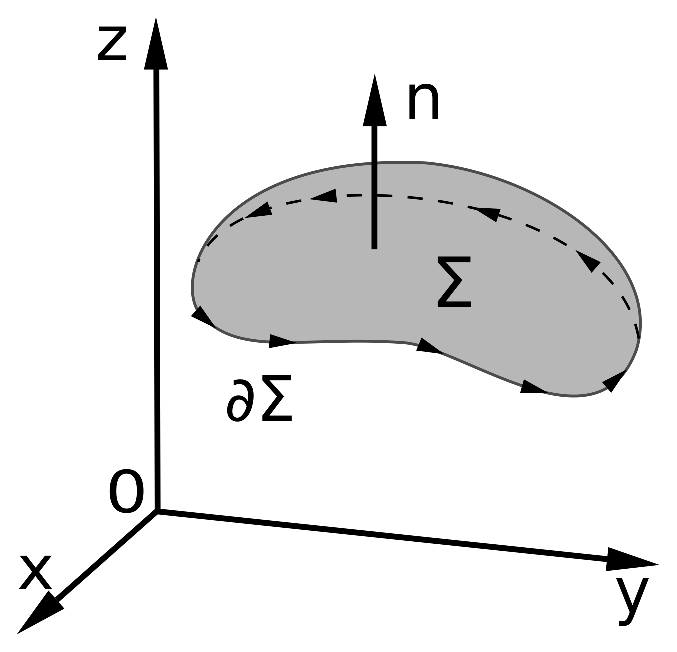
\includegraphics[width=0.7\linewidth]{Immagini/stokes.eps}
        \caption{Here we divide the surface of the sphere in two different surfaces $\mathcal A$ and $\mathcal B$ that share the edge $\mathcal P$}
    \end{figure}
    From the Stokes theorem we have that
    \begin{equation}
        \label{eq:stokes}
            \gamma_n=\oint_\mathcal{P} A^n_\mu\: d\lambda^\mu=\frac 12 \int_\Sigma \Omega_{\mu\nu}^n\: d\lambda^\mu \wedge d\lambda^\nu
    \end{equation}
    where we have used the Einstein convention of summation.\newline
    There is a subtelty in this last equation, as we know the Berry curvature tensor in Gauge-invariant, so the integral over the surface is too, but the integral over the closed path of the Berry connection is defined up to a factor $2n\pi$ that is gauge dependant.
    So is there a modulo $2\pi$ ambiguity or not?\newline
    The answer is that if $\gamma_n$ is to be determined using the knowledge of $\ket{n,\boldsymbol \lambda}$ 
    only on the curve $\mathcal P$ then it is really well defined modulo $2\pi$. In this case we can re-write 
    equation \ref{eq:stokes} as 
    \[
    \frac 12 \int_\Sigma \Omega_{\mu\nu}^n\: d\lambda^\mu \wedge d\lambda^\nu:=\oint_\mathcal{P} A^n_\mu\: d\lambda^\mu
    \]
    Meaning that the integral over the surface $\Sigma$ is equal to \textit{one of the values of} the integrals along the closed path $\mathcal P$\newline

    But what kind of Gauge gives the "correct" answer? If we choose a gauge that is continuous and smooth
    everywhere along the surface $\Sigma$ including on its boundary $\mathcal P$ then equation \ref{eq:stokes} becomes unambiguous.\newline
    While it is possible to make a radical gauge transformation that shifts $\gamma_n$ by $2\pi$ when regarding $\ket{n,\boldsymbol \lambda}$ as a function defined only in the neighborhood of $\mathcal P$, such a gauge change cannot be smoothly continued into the interior $\mathcal S$ without creating a vortex-like singularity of $\gamma_n(\boldsymbol \lambda)$.


\section{Chern Theorem}
    
    Let's take as an example Gauss's theorem. It tells us that the flux of the field through a closed surface is equal to the charges inside. \newline
    Now let's calculate the flux of the Berry curvature through a closed surface. We can divide the closed surface as two different open surfaces that share the same edge $\mathcal P$.\newline
    Thanks to stokes theorem the flux through the surface $\mathcal A$ is $\oint_\mathcal{P} \mathbf A \cdot d\boldsymbol \lambda$, but the flux through the surface $\mathcal B$ is $-\oint_\mathcal{P} \mathbf A \cdot d\boldsymbol \lambda$.\newline
    Theese two integrals must be equal modulo $2\pi$, so
    \begin{figure}
        \centering
        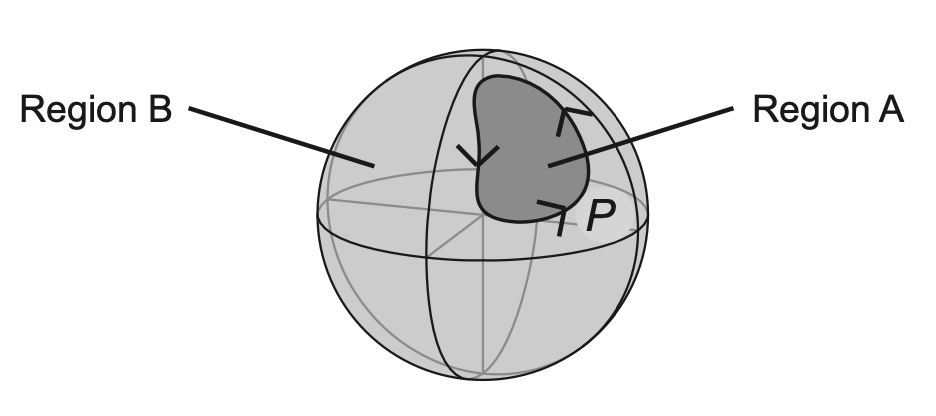
\includegraphics[width=0.85\linewidth]{../website/images/berry/chern_theorem.png}
        \caption{Here we divide the surface of the sphere in two different surfaces $\mathcal A$ and $\mathcal B$ that share the edge $\mathcal P$}
        \label{fig:forward_pass}
    \end{figure}
    \begin{equation}
        \label{eq:chern}
        \oint_\mathcal{S} \Omega_{\mu\nu}^n d\lambda^\mu \wedge d\lambda^\nu =2\pi C \quad\quad C\in \mathbb Z
    \end{equation}
    This means that the flux thought a closed surface of the Berry curvature is quantized
    
    The constant $C$ in known as the Chern number. Note that when the Chern index is nonzero, it is impossible to construct a smooth and continuous gauge over the entire surface $\mathcal{S}$. If such a gauge did exist, then we could apply Stokes’ theorem directly to the entire surface and conclude that the Chern number vanishes, in contradiction with the assumption.\newline
    But what are these "pseudo-charges" inside the closed surface that generate the flux?\newline
    In E.M. a simple way to spot charges (or monopoles) is to look at the fields and see if as some point it diverges as $1/(\mathbf r-\mathbf{r_0})^2$. Let's take a look at $\Omega_{\mu\nu}$ (eq. \ref{eq:berry-curvature3}) and see if we can spot anything similar \footnote{In the equation below I expressed explicitly the $\boldsymbol \lambda$ dependence in the denominator and condensed the formula using the wedge product $\wedge$}
    \begin{equation}
        \label{eq:monopoles1}
        \Omega_{\mu\nu}^n=i\sum_{n'\neq n} \frac{\bra{n}\partial_\mu H\ket{n'}\wedge \bra{n'} \partial_\nu H\ket{n}}
        {\underbrace{[E_{n'}(\boldsymbol \lambda)-E_n(\boldsymbol \lambda)]^2}_
        {\substack{\text{what happens if for some } \boldsymbol \lambda=\boldsymbol \lambda_d  \\\text{ the two energies are the same?}}}}
    \end{equation}
    So, suppose that for some $\boldsymbol \lambda=\boldsymbol \lambda_d$ we have that $E_n (\boldsymbol \lambda_d)=E_m(\boldsymbol \lambda_d)$, now we expand the energies near $\boldsymbol \lambda_d$ at first order
    \[
    \begin{cases}
    E_n(\boldsymbol \lambda)\, \approx E_n(\boldsymbol \lambda_d) +\, \partial_{\boldsymbol \lambda} E_n|_{\boldsymbol \lambda =\boldsymbol \lambda_d}\cdot (\boldsymbol \lambda-\boldsymbol \lambda_d)\\
    E_m(\boldsymbol \lambda)\approx E_n(\boldsymbol \lambda_d) + \partial_{\boldsymbol \lambda} E_m|_{\boldsymbol \lambda =\boldsymbol \lambda_d}\cdot (\boldsymbol \lambda-\boldsymbol \lambda_d)\\

    \end{cases}
    \]
    This means that 
    \[
    E_n(\boldsymbol \lambda)-E_m(\boldsymbol \lambda)\approx \partial_{\boldsymbol \lambda} (E_n-E_m)|_{\boldsymbol \lambda =\boldsymbol \lambda_d}\cdot (\boldsymbol \lambda-\boldsymbol \lambda_d)
    \]
    so the denominator of the berry curvature near $\boldsymbol \lambda_d$ goes like $ 1/(\boldsymbol \lambda-\boldsymbol \lambda_d)^2$.\newline
    This means that there are "charges" or "monopoles" that induce the flux through the closed surface, and they are localized where 2 (or more) energy levels cross
